
 %%%%%%%%%%%%%% practice problems %%%%%%%%%%%

\practiceproblems
\problempart For each of the following sentences identify the quantifier, the subject term, the predicate term, and the copula. Some of these are like the example ``Thirty percent of Canadians speak French'' where the copula is implicit and the predicate needs to be transformed into a noun phrase.

\begin{longtabu}{p{.1\linewidth}p{.9\linewidth}}
\textbf{Example}: & Some dinosaurs had feathers\\
\textbf{Answer}: & Quantifier: Some \\
&Subject term: Dinosaurs \\
&Copula: Implicit \\
& Predicate term: Things with feathers \\
\end{longtabu}

\begin{exercises}
\item Some politicians are not members of tennis clubs.

\answer{
 Quantifier: Some \\
 Subject term: Politicians \\
 Copula: Are \\
 Predicate term: Things that are not members of tennis clubs \\
 }
\item All dogs go to heaven.

\answer{
 Quantifier:  All \\
 Subject term:  Dogs \\
 Copula:  Implicit \\
 Predicate term: Things that go to heaven \\
 }

\item Most things in the fridge are moldy.

\answer{
 Quantifier:  Most \\
 Subject term: Things in the fridge  \\
 Copula:  Are \\
 Predicate term: Things that are moldy  \\
}
\item Some birds do not fly.

\answer{
 Quantifier:  Some \\
 Subject term: Birds \\
 Copula: Implicit \\
 Predicate term: Things that do not fly. \\
 }

\item Few people have seen Janet relaxed and happy.

\answer{
 Quantifier: Few  \\
 Subject term: People \\
 Copula:  Implicit \\
 Predicate term:  People who have seen Janet relaxed and happy. \\
 }
\item No elephants are pocket-sized.

\answer{
 Quantifier: No \\
 Subject term:  Elephants \\
 Copula: Are  \\
 Predicate term: Things that are pocket sized. \\
}
\item Two thirds of Americans are obese or overweight.

\answer{
 Quantifier:  Two thirds \\
 Subject term:  Americans \\
 Copula:  Are\\
 Predicate term: People who are obese or overweight. \\
}
\item All applicants must submit to a background check.

\answer{
 Quantifier:  All \\
 Subject term:  Applicants \\
 Copula:  Implicit \\
 Predicate term:  People who must submit to a background check. \\
 }
\item All handguns are weapons.

\answer{
 Quantifier:  All \\
 Subject term: Handguns  \\
 Copula:  Are\\
 Predicate term: Weapons  \\
 }
\item One man stands alone against injustice.

\answer{
 Quantifier:  One \\
 Subject term:  Man \\
 Copula:  Implicit \\
 Predicate term:  People who stand alone against injustice. \\
 }
\end{exercises}



\noindent \problempart For each of the following sentences identify the quantifier, the subject term, the predicate term, and the copula. Some of these are like the example ``Thirty percent of Canadians speak French'' where the copula is implicit and the predicate needs to be transformed into a noun phrase.


\begin{exercises}
\item No dog has been to Mars.

\answer{
 Quantifier:  No\\
 Subject term:  Dog\\
 Copula:  implicit\\
 Predicate term:  Things that have been to Mars \\
 }

\item All human beings are mortal.

\answer{
 Quantifier:  All\\
 Subject term:  Human beings\\
 Copula:  Are\\
 Predicate term:  Things that are mortal \\
 }

\item Some spears are six feet long.

\answer{
 Quantifier:  Some\\
 Subject term:  Spears \\
 Copula:  Are \\
 Predicate term:  Things that are six feet long \\
 }

\item Most dogs are friendly

\answer{
 Quantifier:  Most\\
 Subject term:  Dogs\\
 Copula:  Are\\
 Predicate term:  Things that are friendly \\
 }

\item Eighty percent of Americans graduate from high school.

\answer{
 Quantifier:  Eighty percent\\
 Subject term:  Americans \\
 Copula:  Implicit\\
 Predicate term:   People who graduate from high school\\
 }

\item Few doctors are poor.

\answer{
 Quantifier:  Few\\
 Subject term:  Doctors\\
 Copula:  Are\\
 Predicate term:   People who are poor\\
 }

\item All squids are cephalopods.

\answer{
 Quantifier:  All\\
 Subject term:  Squids\\
 Copula:  Are \\
 Predicate term:   cephalopods\\
 }

\item No fish can sing.

\answer{
 Quantifier:  No\\
 Subject term:  Fish\\
 Copula:  Implicit\\
 Predicate term:  Things that can sing \\
 }

\item Some songs are sad.

\answer{
 Quantifier:  Some\\
 Subject term:  Songs\\
 Copula:  Are\\
 Predicate term:  Things that are sad \\
 }

\item Two dogs are playing in the backyard.

\answer{
 Quantifier:  Two \\
 Subject term:  Dogs \\
 Copula:  Are \\
 Predicate term:   Things that are playing in the backyard\\
 }

\end{exercises}



%%%%%%%%%%%%%%% Practice problems %%%%%%%%%%

\practiceproblems

\problempart Identify each of the following sentences as A, E, I, or O; state its quantity and quality; and state which terms are distributed. Then draw the Venn Diagram for each.

\begin{longtabu}{p{.1\linewidth}p{.9\linewidth}}
\textbf{Example}: & Some dinosaurs are not herbivores \\
\textbf{Answer}: & Form: O\\
&Quantity: particular \\
&Quality: negative \\
&Terms distributed: $P$ \\
&
%\vspace{.25em}
\noindent 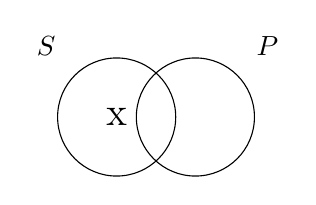
\begin{tikzpicture}
\def\firstcircle{(0,0) circle (.75cm)}
\def\secondcircle{(0:1cm) circle (.75cm)}
\draw \firstcircle node[outer sep=.66cm, above left] (s) {$S$};
\node[outer sep=.3cm] (x) {\Large{x}};
\draw \secondcircle node[outer sep=.66cm, above right] (p) {$P$};
\end{tikzpicture}\\
& $S$: Dinosaurs \\
& $P$: Herbivores
\end{longtabu}

\begin{exercises}

\item All gerbils are rodents.

\answer{
Form: A\\
Quantity: Universal \\
Quality: Affirmative\\
Terms distributed: $S$ \\
\vspace{.25em}

\noindent 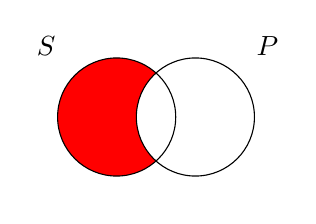
\begin{tikzpicture}
\def\firstcircle{(0,0) circle (.75cm)}
\def\secondcircle{(0:1cm) circle (.75cm)}
       \begin{scope}[even odd rule]% first circle without the second
            \clip \secondcircle (-1,-1) rectangle (1,1);
        \fill[red] \firstcircle;
        \end{scope}
 \draw \firstcircle node[outer sep=.66cm, above left] (s) {$S$};
%\node[outer sep=.3cm] (x) {\Large{x}};
\draw \secondcircle node[outer sep=.66cm, above right] (p) {$P$};
\end{tikzpicture}\\
$S$: Gerbils\\
$P$: Rodents
}

\item Some planets do not have life.

\answer{
Form: O\\
Quantity: Particular \\
Quality: Negative \\
Terms distributed: $P$ \\
\vspace{.25em}
\noindent 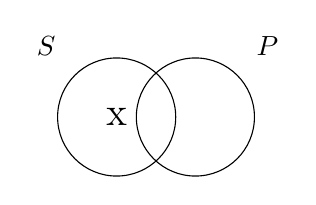
\begin{tikzpicture}
\def\firstcircle{(0,0) circle (.75cm)}
\def\secondcircle{(0:1cm) circle (.75cm)}
\draw \firstcircle node[outer sep=.66cm, above left] (s) {$S$};
\node[outer sep=.3cm] (x) {\Large{x}};
\draw \secondcircle node[outer sep=.66cm, above right] (p) {$P$};
\end{tikzpicture}\\
 $S$: Planets\\
 $P$: Things that have life
}

\item Some manatees are not rappers.

\answer{
Form: O\\
Quantity: Particular \\
Quality: Negative \\
Terms distributed: $P$ \\
\vspace{.25em}
\noindent 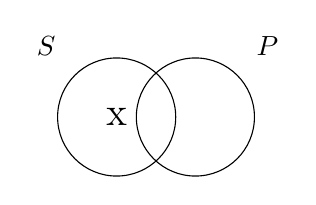
\begin{tikzpicture}
\def\firstcircle{(0,0) circle (.75cm)}
\def\secondcircle{(0:1cm) circle (.75cm)}
\draw \firstcircle node[outer sep=.66cm, above left] (s) {$S$};
\node[outer sep=.3cm] (x) {\Large{x}};
\draw \secondcircle node[outer sep=.66cm, above right] (p) {$P$};
\end{tikzpicture}\\
 $S$: Manatees\\
 $P$: Rappers
}


\item All rooms have televisions.

\answer{
Form: A\\
Quantity: Universal \\
Quality: Affirmative\\
Terms distributed: $S$ \\
\vspace{.25em}

\noindent 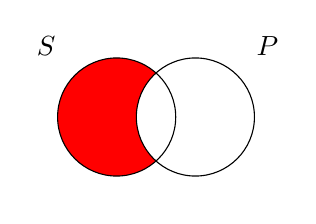
\begin{tikzpicture}
\def\firstcircle{(0,0) circle (.75cm)}
\def\secondcircle{(0:1cm) circle (.75cm)}
       \begin{scope}[even odd rule]% first circle without the second
            \clip \secondcircle (-1,-1) rectangle (1,1);
        \fill[red] \firstcircle;
        \end{scope}
 \draw \firstcircle node[outer sep=.66cm, above left] (s) {$S$};
%\node[outer sep=.3cm] (x) {\Large{x}};
\draw \secondcircle node[outer sep=.66cm, above right] (p) {$P$};
\end{tikzpicture}\\
$S$: Rooms\\
$P$: Things that have televisions
}


\item All stores are closed.

\answer{
Form: A\\
Quantity: Universal \\
Quality: Affirmative\\
Terms distributed: $S$ \\
\vspace{.25em}

\noindent 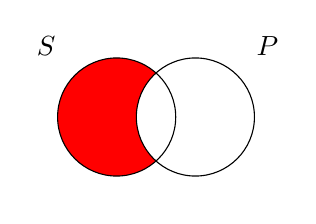
\begin{tikzpicture}
\def\firstcircle{(0,0) circle (.75cm)}
\def\secondcircle{(0:1cm) circle (.75cm)}
       \begin{scope}[even odd rule]% first circle without the second
            \clip \secondcircle (-1,-1) rectangle (1,1);
        \fill[red] \firstcircle;
        \end{scope}
 \draw \firstcircle node[outer sep=.66cm, above left] (s) {$S$};
%\node[outer sep=.3cm] (x) {\Large{x}};
\draw \secondcircle node[outer sep=.66cm, above right] (p) {$P$};
\end{tikzpicture}\\
$S$: Stores\\
$P$: Things that are closed
}


\item Some dancers are graceful.

\answer{
Form: I\\
Quantity: Particular \\
Quality: Affirmative\\
Terms distributed: None \\
\vspace{.25em}

\noindent 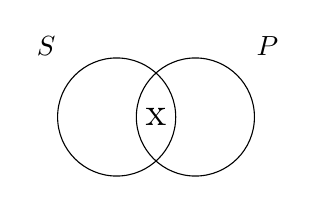
\begin{tikzpicture}
\def\firstcircle{(0,0) circle (.75cm)}
\def\secondcircle{(0:1cm) circle (.75cm)}
%       \begin{scope}[even odd rule]% first circle without the second
%            \clip \secondcircle (-1,-1) rectangle (1,1);
%        \fill[red] \firstcircle;
%        \end{scope}
 \draw \firstcircle node[outer sep=.66cm, above left] (s) {$S$};
%\node[outer sep=.3cm] (x) {\Large{x}};
\node[outer sep=.3cm, xshift=.5cm] (x) {\Large{x}};
\draw \secondcircle node[outer sep=.66cm, above right] (p) {$P$};
\end{tikzpicture}\\
$S$: Dancers\\
$P$: Things that are graceful
}


\item No extraterrestrials are in Cleveland.

\answer{
Form: E\\
Quantity: Universal \\
Quality: Negative\\
Terms distributed: Both \\
\vspace{.25em}

\noindent 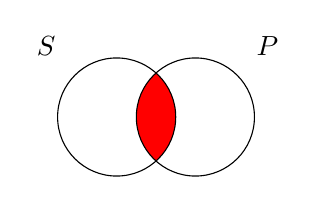
\begin{tikzpicture}
\def\firstcircle{(0,0) circle (.75cm)}
\def\secondcircle{(0:1cm) circle (.75cm)}
%       \begin{scope}[even odd rule]% first circle without the second
%            \clip \secondcircle (-1,-1) rectangle (1,1);
%        \fill[red] \firstcircle;
%        \end{scope}
    \begin{scope}
      \clip \firstcircle;
      \fill[red] \secondcircle;
    \end{scope}
\draw \firstcircle node[outer sep=.66cm, above left] (s) {$S$};
%\node[outer sep=.3cm] (x) {\Large{x}};
%\node[outer sep=.3cm, xshift=.5cm] (x) {\Large{x}};
\draw \secondcircle node[outer sep=.66cm, above right] (p) {$P$};
\end{tikzpicture}\\
$S$: Extraterrestrial\\
$P$: Things in Cleveland
}

\item Some crates are empty.

\answer{
Form: I\\
Quantity: Particular \\
Quality: Affirmative\\
Terms distributed: None \\
\vspace{.25em}

\noindent 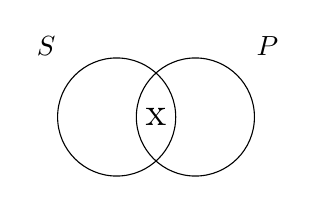
\begin{tikzpicture}
\def\firstcircle{(0,0) circle (.75cm)}
\def\secondcircle{(0:1cm) circle (.75cm)}
%       \begin{scope}[even odd rule]% first circle without the second
%            \clip \secondcircle (-1,-1) rectangle (1,1);
%        \fill[red] \firstcircle;
%        \end{scope}
%    \begin{scope}
%      \clip \firstcircle;
%      \fill[red] \secondcircle;
%    \end{scope}
\draw \firstcircle node[outer sep=.66cm, above left] (s) {$S$};
%\node[outer sep=.3cm] (x) {\Large{x}};
\node[outer sep=.3cm, xshift=.5cm] (x) {\Large{x}};
\draw \secondcircle node[outer sep=.66cm, above right] (p) {$P$};
\end{tikzpicture}\\
$S$: Crates\\
$P$: Things that are empty
}



\item No customers are mistaken.


\answer{
Form: E\\
Quantity: Universal \\
Quality: Negative\\
Terms distributed: Both\\
\vspace{.25em}

\noindent 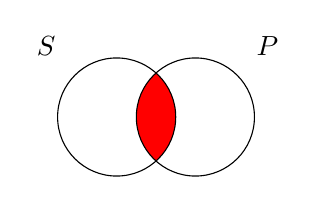
\begin{tikzpicture}
\def\firstcircle{(0,0) circle (.75cm)}
\def\secondcircle{(0:1cm) circle (.75cm)}
%       \begin{scope}[even odd rule]% first circle without the second
%            \clip \secondcircle (-1,-1) rectangle (1,1);
%        \fill[red] \firstcircle;
%        \end{scope}
    \begin{scope}
      \clip \firstcircle;
      \fill[red] \secondcircle;
    \end{scope}
\draw \firstcircle node[outer sep=.66cm, above left] (s) {$S$};
%\node[outer sep=.3cm] (x) {\Large{x}};
%\node[outer sep=.3cm, xshift=.5cm] (x) {\Large{x}};
\draw \secondcircle node[outer sep=.66cm, above right] (p) {$P$};
\end{tikzpicture}\\
$S$: Customers\\
$P$: Things that are mistaken}


\item All cats love catnip.

\answer{
Form: A\\
Quantity: Universal \\
Quality: Affirmative\\
Terms distributed: $S$ \\
\vspace{.25em}

\noindent 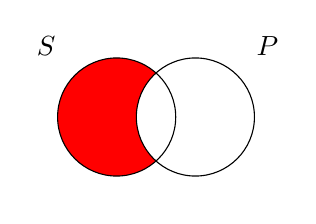
\begin{tikzpicture}
\def\firstcircle{(0,0) circle (.75cm)}
\def\secondcircle{(0:1cm) circle (.75cm)}
       \begin{scope}[even odd rule]% first circle without the second
            \clip \secondcircle (-1,-1) rectangle (1,1);
        \fill[red] \firstcircle;
        \end{scope}
%    \begin{scope}
%      \clip \firstcircle;
%      \fill[red] \secondcircle;
%    \end{scope}
\draw \firstcircle node[outer sep=.66cm, above left] (s) {$S$};
%\node[outer sep=.3cm] (x) {\Large{x}};
%\node[outer sep=.3cm, xshift=.5cm] (x) {\Large{x}};
\draw \secondcircle node[outer sep=.66cm, above right] (p) {$P$};
\end{tikzpicture}\\
$S$: Cats\\
$P$: Things that love catnip
}

\end{exercises}

\noindent \problempart Identify each of the following sentences as A, E, I, or O; state its quantity and quality; and state which terms are distributed. Then draw the Venn Diagram for each.

\begin{exercises}


\item No appeals are rejected.



\item All bagels are boiled.

\item Some employees are late.

\item All forgeries are discovered eventually.

\item Some shirts are purple.

\item Some societies are matriarchal.

\item No sunflowers are blue.

\item Some appetizers are filling.

\item Some jokes are funny.

\item Some arguments are invalid.

\end{exercises}

\noindent\problempart Transform the following sentences by switching their quantity, but not their quality.

\textbf{Example}: Some dogs have fleas. \\
\textbf{Answer}: All dogs have fleas.

\begin{exercises}
\item Some trees are not evergreen. \answer{ No trees are evergreen}
\item All smurfs are blue. \answer{ Some smurfs are blue}
\item Some swords are sharp. \answer{ All swords are sharp}
\item Some sweaters are not soft. \answer{ No sweaters are soft}
\item All snails are invertebrates. \answer{Some snails are invertebrates}
\end{exercises}

\noindent\problempart Transform the following sentences by switching their quantity, but not their quality.

\begin{exercises}
\item Some puffins are not large.
\item Some Smurfs are female.
\item All guitars are stringed instruments.
\item No lobsters are extraterrestrial.
\item Some metals are alloys
\end{exercises}

\noindent\problempart Transform the following sentences by switching their quality, but not their quantity.

\textbf{Example}: Some elephants are in zoos. \\
\textbf{Answer}: Some elephants are not in zoos.

\begin{exercises}
\item Some lobsters are white. \answer{Some lobsters are not white.}

\item Some responsibilities are onerous. \answer{ Some responsibilities are not onerous}

\item No walls are bridges. \answer{All walls are bridges}

\item Some riddles are not clever.\answer{ Some riddles are clever}

\item All red things are colored. \answer{No red things are colored}
\end{exercises}

\noindent\problempart Transform the following sentences by switching their quality, but not their quantity.

\begin{exercises}
\item All drums are musical instruments.
\item No grandsons are female.
\item Some crimes are felonies.
\item Some airplanes are not commercial.
\item All scorpions are arachnids.
\end{exercises}

\noindent\problempart Transform the following sentences by switching both their quality and quantity.

\textbf{Example}: No sharks are virtuous. \\
\textbf{Answer}: Some sharks are virtuous.

\begin{exercises}
\item No lobsters are vertebrates. \answer{Some lobsters are vertebrates}

\item Some colors are not pastel. \answer{All colors are pastel}

\item All tents are temporary structures.\answer{Some tents are not temporary structures}

\item No goats are bipeds. \answer{Some goats are bipeds}

\item Some shirts are plaid.\answer{ No shirts are plaid}
\end{exercises}

\noindent\problempart Transform the following sentences by switching both their quality and quantity.

\begin{exercises}
\item No shirts are pants.
\item All ducks are birds.
\item Some possibilities are not likely events.
\item Some raincoats are blue.
\item Some days are holidays.
\end{exercises}





%%%%%%%%%% practice problems %%%%%%%%%%%%

\practiceproblems
\noindent\problempart Transform the following into logically structured English; identify it as A, E, I, or O; and provide the appropriate Venn diagram.


\begin{longtabu}{p{.1\linewidth}p{.9\linewidth}}
\textbf{Example}: & If you can't stand the heat, get out of the kitchen \\
\textbf{Answer}:  & All people who cannot stand the heat are people who should get out of the kitchen. \\
& Form: A\\
&
\noindent 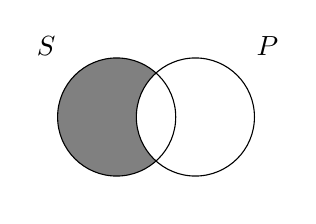
\begin{tikzpicture}
\def\firstcircle{(0,0) circle (.75cm)}
\def\secondcircle{(0:1cm) circle (.75cm)}
     \begin{scope}[shift={(4cm,0cm)}]
        \begin{scope}[even odd rule]% first circle without the second
            \clip \secondcircle (-1,-1) rectangle (1,1);
        \fill[gray] \firstcircle;
        \end{scope}
\draw \firstcircle node[outer sep=.66cm, above left] (s) {$S$};
\draw \secondcircle node[outer sep=.66cm, above right] (p) {$P$};
        \end{scope}

\end{tikzpicture}\\
& $S$: People who can't stand the heat\\
& $P$: People who should get out of the kitchen

\end{longtabu}

\begin{exercises}

\item If something is worth doing, it is worth doing well. \answer{\\
All things that are worth doing are things that are worth doing well. \\
Form: A \\
\begin{venns}
\MoodAStatementRed
\end{venns}

$S$: Things that are worth doing \\
$P$: Things that are worth doing well.
}

\item Cats are not herbivores.\answer{\\
No cats are herbivores. \\
Form: E \\
\begin{venns}
\MoodEStatementRed
\end{venns}

$S$: Cats\\
$P$: Herbivores
}

\item Some chimpanzees know sign language. \answer{\\
Some chimpanzees are things that know sign language. \\
Form: I \\
\begin{venns}
\MoodIStatementRed
\end{venns}

$S$: Chimpanzees \\
$P$: Things that know sign language.
}

\item Some dogs are not loyal. \answer{\\
Some dogs are not things that are loyal. \\
Form: O \\
\begin{venns}
\MoodOStatementRed
\end{venns}

$S$: Dogs \\
$P$: Things that are loyal.
}

\item Monotremes are the only egg-laying mammals.\answer{\\
All egg-laying mammals are monotremes. \\
Form: A \\
\begin{venns}
\MoodAStatementRed
\end{venns}

$S$: Egg-laying mammals \\
$P$: Monotremes\\
\vspace{11pt}
Remember that ``the only'' introduces the subject, not the predicate.
}

\item Whenever a bell rings, an angel gets its wings. \answer{\\
All times that a bell rings are times that an angel gets its wings. \\
Form: A \\
\begin{venns}
\MoodAStatementRed
\end{venns}

$S$: Times that a bell rings \\
$P$: Times that an angel gets its wings\\
\vspace{11pt}
Remember that words like ``whenever'' and ``where ever'' are really specialized quantifiers for places and times, and need to be replaced by ``all places'' and ``all times.'' See page 71.
}


\item At least one person in this room is a liar. \answer{\\
Some people in this room are liars. \\
Form: I \\
\begin{venns}
\MoodIStatementRed
\end{venns}

$S$: People in this room \\
$P$: Liars\\
\vspace{11pt}
}


\item Only natural born citizens can be president of the United States.\answer{\\
All presidents of the United States are natural born citizens. \\
Form: A \\
\begin{venns}
\MoodAStatementRed
\end{venns}

$S$: Presidents of the United States\\
$P$: Natural born citizens\\
\vspace{11pt}
}

\item Gottlob Frege suffered from severe depression. \answer{\\
All people identical with Gottlob Frege are people who suffer from severe depression. \\
Form: A \\
\begin{venns}
\MoodAStatementRed
\end{venns}

$S$: People identical with Gottlob Frege\\
$P$: People who suffer from severe depression\\
}

\item ``Anyone who ever had a heart, wouldn't turn around and break it.'' --Lou Reed. \answer{\\
No things who ever had a heart are things that would turn around and break it. \\
Form: E \\

\begin{venns}
\MoodEStatementRed
\end{venns}

$S$: Things who ever had a heart\\
$P$: Things that would turn around a break it\\
}

\end{exercises}

\noindent\problempart Transform the following into logically structured English; identify it as A, E, I, or O; and provide the appropriate Venn diagram.

\begin{exercises}
\item If a muffin has frosting, then it is a cupcake. \answer{\\
All muffins with frosting are cupcakes\\
Mood: A\\
\begin{venns}
\MoodAStatementRed
\end{venns}

$S$: Muffins with frosting\\
$P$: Cupcakes\\
}

\item Some birds eat fish. \answer{\\
Some birds are things that eat fish \\
Mood: I\\
\begin{venns}
\MoodIStatementRed
\end{venns}\\
$S$: Birds\\
$P$: Things that eat fish\\
}

\item Dragons don't take kindly to strangers \answer{\\
No dragons are things that take kindly to strangers.\\
Mood: E\\
\begin{venns}
\MoodEStatementRed
\end{venns}\\
$S$:  Dragons\\
$P$:  Things that take kindly to strangers\\
}

\item Some logicians are not mentally ill \answer{\\
Some logicians are not people who are mentally ill\\
Mood: O\\
\begin{venns}
\MoodOStatementRed
\end{venns}\\
$S$:  Logicians\\
$P$:  People who are not mentally ill\\
}

\item There's no milk in the fridge \answer{\\
No things in the fridge are milk \\
Mood: E\\
\begin{venns}
\MoodEStatementRed
\end{venns}\\
$S$:  Things in the fridge\\
$P$:  Milk\\
}

\item Seahorses are the only fish species in which the male carries the babies. \answer{\\
All fish species where the male carries the babies are seahorses   \\
Mood: A\\
\begin{venns}
\MoodAStatementRed
\end{venns}\\
$S$:  Fish species where the male carries the babies\\
$P$:  Seahorses\\
}

\item Seahorses are animals that mate for life. \answer{\\
 All seahorses are animals that made for life  \\
Mood:  A\\
\begin{venns}
\MoodAStatementRed
\end{venns} \\
$S$:  Seahorses\\
$P$:  Animals that mate for life\\
}

\item Few dogs are fans of classical music. \answer{\\
Some dogs are fans of classical music   \\
Mood:  I\\
\begin{venns}
\MoodIStatementRed
\end{venns}\\
$S$:  Dogs\\
$P$:  Fans of classical music\\
}

\item Ruth Barcan Marcus was a member of the Yale faculty. \answer{\\
 All people identical to Ruth Barcan Marcus were members of the Yale faculty  \\
Mood: A \\
\begin{venns}
\MoodAStatementRed
\end{venns}\\
$S$:  People identical to Ruth Barcan Marcus \\
$P$:  Members of the Yale faculty  \\
}

\item Only zombies are brain eaters. \answer{\\
 All brain eaters are zombies  \\
Mood:  A \\
\begin{venns}
\MoodAStatementRed
\end{venns}\\
$S$:  Brain eaters\\
$P$:  Zombies\\
}

\end{exercises}

\noindent\problempart Transform the following into logically structured English; identify it as A, E, I, or O; and provide the appropriate Venn diagram. Some problems will require multiple transformations.

\begin{longtabu}{p{.1\linewidth}p{.9\linewidth}}
\textbf{Example}: & Bertrand Russell was married four times. \\
\textbf{Answer}:  & All people who are identical to Bertrand Russell are people who were married four times. \\
& Form: A\\
&
\noindent 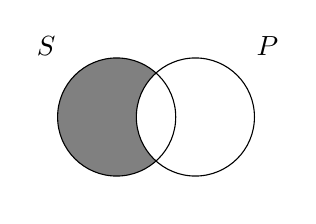
\begin{tikzpicture}
\def\firstcircle{(0,0) circle (.75cm)}
\def\secondcircle{(0:1cm) circle (.75cm)}
     \begin{scope}[shift={(4cm,0cm)}]
        \begin{scope}[even odd rule]% first circle without the second
            \clip \secondcircle (-1,-1) rectangle (1,1);
        \fill[gray] \firstcircle;
        \end{scope}
\draw \firstcircle node[outer sep=.66cm, above left] (s) {$S$};
\draw \secondcircle node[outer sep=.66cm, above right] (p) {$P$};
        \end{scope}
\end{tikzpicture}\\
& $S$: People who are identical to Bertrand Russell\\
& $P$: People who were married four times
\end{longtabu}

\begin{exercises}

\item Many logicians work in computer science. \answer{\\
Some logicians are people who work in computer science. \\
Form: I \\
\begin{venns}
\MoodIStatementRed
\end{venns}\\
$S$: Logicians\\
$P$: People that work in computer science\\
}


\item Ludwig Wittgenstein served in the Austro-Hungarian Army in World War I.\answer{\\
All people identical to Ludwig Wittgenstein are people that served in the Austro-Hungarian Army in World War I \\
Form: A \\
\begin{venns}
\MoodAStatementRed
\end{venns}\\
$S$: People identical to Ludwig Wittgenstein\\
$P$: People that served int he Austro-Hungarian Army in WWI\\
}

\item Martians can be found nowhere on Earth.\answer{\\
No place on earth is a place where you can find Martians. \\
Form: E \\
\begin{venns}
\MoodEStatementRed
\end{venns}\\
$S$: Places on Earth\\
$P$: Places you can find Martians\\
}

\item One of our cats is not awake. \answer{\\
Some of our cats are not animals that are awake\\
Form: O \\
\begin{venns}
\MoodOStatementRed
\end{venns}\\
$S$: Our cats\\
$P$: Animals that are awake\\
}

\item Grover Cleveland was the only president to serve two nonconsecutive terms. \answer{\\
All presidents who served two nonconsecutive terms are people identical to Grover Cleveland. \\
Form: A \\
\begin{venns}
\MoodAStatementRed
\end{venns}\\
$S$: Presidents who served two nonconsecutive terms \\
$P$: People identical to Grover Cleveland\\
}

\item Grover Cleveland was not a Muppet \answer{\\
No people identical to Grover Cleveland are Muppets \\
Form: E \\
\begin{venns}
\MoodEStatementRed
\end{venns}\\
$S$: People identical to Grover Cleveland\\
$P$: Muppets\\
}



\item The band's only singer also plays guitar. \answer{\\
All people identical to the singer of the band are people who play guitar. \\
Form: A \\
\begin{venns}
\MoodAStatementRed
\end{venns}\\
$S$: People identical to the singer of the band\\
$P$: People who play guitar\\
}

\item If a dog has a collar, it is someone's pet.\answer{\\
All dogs that have a collar are animals that are someone's pet.\\
Form: A \\
\begin{venns}
\MoodAStatementRed
\end{venns}\\
$S$: Dogs that have a collar\\
$P$: Animals that are someone's pet. \\
}

\item Only the basketball players in the class were tall. \answer{\\
All tall people in the class were basketball players\\
Form: A \\
\begin{venns}
\MoodAStatementRed
\end{venns}\\
$S$: Tall people in the class\\
$P$: Basketball players\\
}

\item If you study, then you will not fail the test.\answer{\\
No people who study are people who will fail the test. \\
Form: E \\
\begin{venns}
\MoodEStatementRed
\end{venns}\\
$S$: People who study \\
$P$: People who fail the test\\
}

\end{exercises}


\noindent\problempart Transform the following into logically structured English; identify it as A, E, I, or O; and provide the appropriate Venn diagram. Some problems will require multiple transformations.

\begin{exercises}
\item People have walked on the moon at least once.
\item Basketball players are tall.
\item Most senior citizens vote.
\item If a bird is a crow, then it is very intelligent.
\item Whoever ate the last cookie is in trouble.
\item ``Euclid alone has looked on Beauty bare.'' --Edna St. Vincent Millay.
\item If something is a dog, then it is man's best friend.
\item More than a few students will fail the test.
\item Mercury is the only metal that is liquid at room temperature.
\item Bertrand Russell was married four times.
\end{exercises}

%Something is a dog only if it's not a cat.
%Dogs are not cats. &
%No dogs are cats.\\






%%%%%%%%%%%%%%%%%%%%% practice problems %%%%%%%%%%%%%

\practiceproblems

\noindent \problempart For each sentence, write the converse, obvserse, or contrapostive as directed.

\begin{longtabu}{p{.1\linewidth}p{.9\linewidth}}
\textbf{Example}: & Write the contrapositive of ``Some sentences are categorical.''\\
\textbf{Answer}: & Some non-categorical things are non-sentences. \\
\end{longtabu}

\begin{exercises}
\item Write the converse of ``No weeds are benign.''
\answer{\\No benign things are weeds}

\item Write the converse of ``Some minds are not closed.''
\answer{\\Some closed things are not minds}

\item Write the contraposition of ``Some dentists are underpaid.''
\answer{\\Some non-underpaid people are non-dentists}

\item Write the converse of ``All humor is good.''
\answer{\\All good things are humorous}

\item Write the contraposition of ``No organizations are self-sustaining.''
\answer{\\No non-self-sustaining things are non-organizations}

\item Write the obverse of ``Some dogs have fleas.''
\answer{\\Some dogs are not non-flea-havers. \\
or Some dogs are not non-flea-having things.}

\item Write the converse of ``Some things that have fleas are dogs.''
\answer{\\Some dogs have fleas}

\item Write the obverse of ``No detectives are uniformed.''
\answer{\\All detectives are ununiformed. }

\item Write the converse of ``No monkeys are well-behaved.''
\answer{\\No well-behaved things are monkeys"}

\item Write the contraposition of ``No donkeys are obedient.''
\answer{\\No disobedient things are non-donkeys." }

\end{exercises}

\noindent \problempart For each sentence, write the converse, obvserse, or contrapostive as directed.
\begin{exercises}
\item Write the converse of ``No supplies are limited.''
\item Write the obverse of ``No knives are toys.''
\item Write the contraposition of ``All logicians are rational.''
\item Write the obverse of ``All uniforms are clothing.''
\item Write the converse of ``All risks are negligible.''
\item Write the contraposition of ``No bestsellers are great works of literature.''
\item Write the obverse of ``Some descriptions are accurate.''
\item Write the contraposition of ``Some ties are not tacky.''
\item Write the obverse of ``All spies are concealed.''
\item Write the contraposition of ``No valleys are barren.''
\end{exercises}


\problempart The first two columns in the table below give you a statement and a truth value for that statement. The next column gives an operation that can be performed on the statement in the first column, and the final two columns give the new statement and its truth value.

The first row is completed, as an example, but after that there are blanks. In problems 1--5 you must fill in the new statement and its truth value, and in problems 6--10 you must fill in the operation and the final truth value. If the truth value of the resulting statement cannot be determined from the original one, write a ``?'' for ``undetermined.'' You can check your work with Venn diagrams, or by identifying the logical form of the original statement and seeing if it is one where the named operation changes the truth value.

\begin{longtabu}{X[1,l,m]X[15,l,m]X[2,l,m]X[6,l,m]X[16,l,m]X[1,l,m]}
%{p{.01\linewidth}p{.2\linewidth}p{.15\linewidth}p{.15\linewidth}p{.2\linewidth}p{.1\linewidth}}
%{llllll}
 & \underline{Given statement} & \underline{T/F} & \underline{Operation} & \underline{New Statement} & \underline{T/F/?} \\
  \rowcolor{light-gray}
 Ex. & All $S$ are $P$ & F & Conv. & All $P$ are $S$ & ? \\
 \endhead

1. & Some $S$ are $P$  & F  & Obv. & \answer{Some $S$ are not non-$P$}{\rule[-5pt]{2.5cm}{.4pt}}& \answer{F}{\rule[-5pt]{.5cm}{.4pt}}\\



2.& Some non-$S$ are $P$  & F& Conv. & \answer{Some $P$ are non-$S$}{\rule[-5pt]{2.5cm}{.4pt}}&\answer{F}{\rule[-5pt]{.5cm}{.4pt}}\\


3. & All $S$ are $P$  & F & Contrap. & \answer{All non-$P$ are non-$S$}{\rule[-5pt]{2.5cm}{.4pt}}& \answer{F}{\rule[-5pt]{.5cm}{.4pt}}\\

4. & Some $S$ are $P$  & F & Contrap. & \answer{Some non-$P$ are non-$S$}{\rule[-5pt]{2.5cm}{.4pt}}& \answer{?}{\rule[-5pt]{.5cm}{.4pt}}\\

5. & Some $S$ are non-$P$ & T & Obv. & \answer{Some $S$ are not $P$}{\rule[-5pt]{2.5cm}{.4pt}}& \answer{T}{\rule[-5pt]{.5cm}{.4pt}}\\

6.& All $S$ are non-$P$  & T & \answer{Contrap.}{\rule[-5pt]{1.5cm}{.4pt}}& All $P$ are non-$S$ & \answer{T}{\rule[-5pt]{.5cm}{.4pt}}\\

7.& Some non-$S$ are not P & T & \answer{Conv.}{\rule[-5pt]{1.5cm}{.4pt}}& Some $P$ are not non-$S$ & \answer{?}{\rule[-5pt]{.5cm}{.4pt}}\\

8. & Some $S$ are not P & F  & \answer{Conv.}{\rule[-5pt]{1.5cm}{.4pt}}& Some $P$ are not $S$ & \answer{?}{\rule[-5pt]{.5cm}{.4pt}}\\

9.& All non-$S$ are $P$ & T & \answer{Obv.}{\rule[-5pt]{1.5cm}{.4pt}}& No non-$S$ are non-$P$ & \answer{T}{\rule[-5pt]{.5cm}{.4pt}}\\

10. & No non-$S$ are non-$P$ & T & \answer{Obv.}{\rule[-5pt]{1.5cm}{.4pt}} & All non-$S$ are non-non-$P$ & \answer{T}{\rule[-5pt]{.5cm}{.4pt}}\\

\end{longtabu}

\problempart See the instructions for Part A.

\begin{longtabu}{X[1,l,m]X[15,l,m]X[2,l,m]X[6,l,m]X[16,l,m]X[1,l,m]}
%{p{.01\linewidth}p{.2\linewidth}p{.15\linewidth}p{.15\linewidth}p{.2\linewidth}p{.1\linewidth}}
%{llllll}
 & \underline{Given statement} & \underline{T/F} & \underline{Operation} & \underline{New Statement} & \underline{T/F} \\



1. & All $S$ are $P$& T & Obv. & \nix{ } \rule[-5pt]{2.5cm}{.4pt}  & \nix{ } \rule[-5pt]{.5cm}{.4pt} \\

2.& Some $S$ are not non-$P$& T & Contrap. & \nix{ } \rule[-5pt]{2.5cm}{.4pt} &\nix{ } \rule[-5pt]{.5cm}{.4pt} \\


3. & No $S$ are non-$P$& T & Obv. & \nix{  } \rule[-5pt]{2.5cm}{.4pt} & \nix{ } \rule[-5pt]{.5cm}{.4pt} \\

4. & All non-$S$ are $P$& T & Obv. & \nix{ } \rule[-5pt]{2.5cm}{.4pt}& \nix{ } \rule[-5pt]{.5cm}{.4pt} \\

5. & Some non-$S$ are $P$& F & Contrap. & \nix{ } \rule[-5pt]{2.5cm}{.4pt}& \nix{ } \rule[-5pt]{.5cm}{.4pt} \\

6. & Some $S$ are $P$& F &  \nix{Obv.} \rule[-5pt]{1.5cm}{.4pt} & Some $S$ are not non-$P$  & \nix{F} \rule[-5pt]{.5cm}{.4pt} \\

7.& No non-$S$ are non-$P$& F &  \nix{Contrap.} \rule[-5pt]{1.5cm}{.4pt} & No $P$ are $S$  & \nix{?}\rule[-5pt]{.5cm}{.4pt} \\

8. & Some non-$S$ are non-$P$& T & \nix{Contrap.} \rule[-5pt]{1.5cm}{.4pt} & Some $P$ are $S$ & \nix{?} \rule[-5pt]{.5cm}{.4pt} \\

9.& All $S$ are $P$ & F & \nix{Obv.}\rule[-5pt]{1.5cm}{.4pt}  & No $S$ are non-$P$  & \nix{F} \rule[-5pt]{.5cm}{.4pt} \\

10. &  Some non-$S$ are not non-$P$ &  T & \nix{Obv.} \rule[-5pt]{1.5cm}{.4pt}  &Some non-$S$ are $P$   & \nix{T}  \rule[-5pt]{.5cm}{.4pt} \\
 \end{longtabu}


\noindent \problempart Determine whether the following arguments are valid by drawing a Venn diagram for the premise. If they are valid, say whether they are valid by conversion, obversion, or contraposition.

\begin{longtabu}{p{.2\linewidth}p{.8\linewidth}}
\textbf{Example 1}: & All swans are white. Therefore, no swans are non-white.\\
\textbf{Answer}: & \\
&\noindent 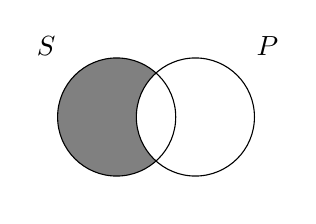
\begin{tikzpicture}
\def\firstcircle{(0,0) circle (.75cm)}
\def\secondcircle{(0:1cm) circle (.75cm)}
     \begin{scope}[shift={(4cm,0cm)}]
        \begin{scope}[even odd rule]% first circle without the second
            \clip \secondcircle (-1,-1) rectangle (1,1);
        \fill[gray] \firstcircle;
        \end{scope}
\draw \firstcircle node[outer sep=.66cm, above left] (s) {$S$};
\draw \secondcircle node[outer sep=.66cm, above right] (p) {$P$};
        \end{scope}
\end{tikzpicture}\\
& $S$: Swans \\
&$P$: White things. \\
& Valid, because the Venn diagram for the premise also makes the conclusion true.\\
& Obversion.\\
\end{longtabu}

\begin{longtabu}{p{.2\linewidth}p{.8\linewidth}}
\textbf{Example 2}: & Some dogs are pets. Therefore, some non-pets are non-dogs. \\
\textbf{Answer}: & \\
&\noindent 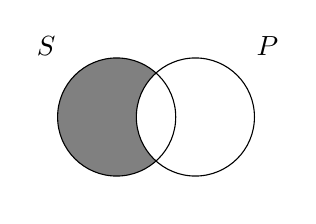
\begin{tikzpicture}
\def\firstcircle{(0,0) circle (.75cm)}
\def\secondcircle{(0:1cm) circle (.75cm)}
     \begin{scope}[shift={(4cm,0cm)}]
        \begin{scope}[even odd rule]% first circle without the second
            \clip \secondcircle (-1,-1) rectangle (1,1);
        \fill[gray] \firstcircle;
        \end{scope}
\draw \firstcircle node[outer sep=.66cm, above left] (s) {$S$};
\draw \secondcircle node[outer sep=.66cm, above right] (p) {$P$};
        \end{scope}
\end{tikzpicture}\\
& $S$: Pets\\
&$P$: Dogs. \\
& Invalid, because the Venn diagram for the premise doesn't make the conclusion true.\\
\end{longtabu}

\begin{exercises}
\item Some smurfs are not blue. Therefore, some blue things are not smurfs.

\answer{
\begin{venns}
\someexistonesent
\drawsubsent
\drawpredsent
\end{venns}\\

S: Smurfs \\
P: Blue things\\
Invalid, because the Venn diagram for the premise does not make the conclusion true. }

\item All giraffes are majestic. Therefore, all non-majestic things are non-giraffes.

\answer{
\begin{venns}
%\someexistonesent
\shadecomplementred{\subjectcircle}{\subjectsquare}{\predicatecircle}
\drawsubsent
\drawpredsent
\end{venns}\\
S: Giraffes\\
P: Majestic things\\
Valid, because the diagram for the premise is also the diagram for the conclusion.\\
Contraposition on a mood-A statement

}


\item Some roosters are not pets.	Therefore, some pets are not roosters.

\answer{
\begin{venns}
\someexistonesent
%\shadecomplementred{\subjectcircle}{\subjectsquare}{\predicatecircle}
\drawsubsent
\drawpredsent
\end{venns}\\
S: Roosters\\
P: Pets\\
%Valid, because the diagram for the premise is also the diagram for the conclusion.
Invalid, because the Venn diagram for the premise does not make the conclusion true.
 }

\item No anesthesiologists are doctors. Therefore, no doctors are anesthesiologists.

\answer{
\begin{venns}
%\someexistonesent
%\shadecomplementred{\subjectcircle}{\subjectsquare}{\predicatecircle}
\shadeintersectred{\subjectcircle}{\predicatecircle}
\drawsubsent
\drawpredsent
\end{venns}\\
S: Anesthesiologists\\
P: Soctors\\
Valid, because the diagram for the premise is also the diagram for the conclusion.
%Invalid, because the Venn diagram for the premise does not make the conclusion true.
Conversion on a mood-E statement.
}

\item All penguins are flightless. Therefore, all flightless things are penguins.

\answer{
\begin{venns}
%\someexistonesent
\shadecomplementred{\subjectcircle}{\subjectsquare}{\predicatecircle}
%\shadeintersectred{\subjectcircle}{\predicatecircle}
\drawsubsent
\drawpredsent
\end{venns}\\
S: Penguins\\
P: Flightless things \\
%Valid, because the diagram for the premise is also the diagram for the conclusion.
Invalid, because the Venn diagram for the premise does not make the conclusion true.
%Conversion.
}

\item No kisses are innocent. Therefore, no non-innocent things are non-kisses.

\answer{
\begin{venns}
%\someexistonesent
%\shadecomplementred{\subjectcircle}{\subjectsquare}{\predicatecircle}
\shadeintersectred{\subjectcircle}{\predicatecircle}
\drawsubsent
\drawpredsent
\end{venns}\\
S: Kisses\\
P: Innocent things\\

%Invalid, because the Venn diagram for the premise does not make the conclusion true.
Contraposition on a mood-E statement.
}

\item All operas are sung. Therefore, all sung things are operas.

\answer{
\begin{venns}
%\someexistonesent
\shadecomplementred{\subjectcircle}{\subjectsquare}{\predicatecircle}
%\shadeintersectred{\subjectcircle}{\predicatecircle}
\drawsubsent
\drawpredsent
\end{venns}\\
S: Operas \\
P: Things that are sung\\
%Valid, because the diagram for the premise is also the diagram for the conclusion.
Invalid, because the Venn diagram for the premise does not make the conclusion true.
}
\item Some shopping malls are not abandoned. Therefore, some shopping malls are non-abandoned.
\answer{
\begin{venns}
\someexistonesent
%\shadecomplementred{\subjectcircle}{\subjectsquare}{\predicatecircle}
%\shadeintersectred{\subjectcircle}{\predicatecircle}
\drawsubsent
\drawpredsent
\end{venns}\\
S: \\
P: \\
Valid, because the diagram for the premise is also the diagram for the conclusion.\\
%Invalid, because the Venn diagram for the premise does not make the conclusion true.
Obversion--always valid}

\item Some great-grandfathers are not deceased. Therefore, some non-deceased people are not non-great-grandfathers.

\answer{
\begin{venns}
\someexistonesent
\drawsubsent
\drawpredsent
\end{venns}\\
S: Great-grandfathers\\
P: Deceased people\\
Valid, because the diagram for the premise is also the diagram for the conclusion. \\
%Invalid, because the Venn diagram for the premise does not make the conclusion true.
Contraposition on an O statement.
}

\item Some boats are not seaworthy. Therefore, some boats are non-seaworthy.

\answer{
\begin{venns}
\someexistonesent
%\shadecomplementred{\subjectcircle}{\subjectsquare}{\predicatecircle}
%\shadeintersectred{\subjectcircle}{\predicatecircle}
\drawsubsent
\drawpredsent
\end{venns}\\
S: Boats\\
P: Seaworthy things\\
Valid, because the diagram for the premise is also the diagram for the conclusion.\\
%Invalid, because the Venn diagram for the premise does not make the conclusion true.
Obversion--always valid.
}
\end{exercises}


\noindent \problempart Determine whether the following arguments are valid by drawing a Venn diagram for the premise. If they are valid, say whether they are valid by conversion, obversion, or contraposition.

\begin{exercises}
\item No platypuses are spies. Therefore, no non-platypuses are non-spies.
\item All sunburns are painful. Therefore, all painful things are sunburns.
\item All ghosts are friendly. Therefore, all non-friendly things are non-ghosts.
\item Some philosophers are not logicians. Therefore, some philosophers are non-logicians.
\item Some felines are lions. Therefore, some felines are not non-lions.
\item No doubts are unreasonable. Therefore, no reasonable things are non-doubts.
\item All Mondays are weekdays. Therefore, no Mondays are non-weekdays.
\item Some colors are pastels. Therefore, some pastel things are colors.
\item All dogs are cosmonauts. Therefore, all cosmonauts are dogs.
\item All cobwebs are made of spider silk. 	Therefore, no cobwebs are made of non-spider silk.
\end{exercises}



%%%%%%%%%%%%%%%%%%%% Practice Problems %%%%%

\practiceproblems
\noindent \problempart For each pair of sentences say whether they are contradictories, contraries, subcontraries, or one is the subaltern of the other.

\begin{longtabu}{p{.1\linewidth}p{.9\linewidth}}
\textbf{Example}: & Some peppers are spicy. \newline No peppers are spicy. \\
\textbf{Answer}: &Contradictory\\
\end{longtabu}

\begin{exercises}

\item No quotations are spurious. \answer{(E)} \\
	Some quotations are not spurious. \answer{(O)} \answer{\\The second is subaltern to the first.}

\item Some children are not picky eaters. \answer{(O)} \\
	All children are picky eaters. \answer{(A)}\answer{\\Contradictories}

\item Some joys are not fleeting. \answer{(O)} \\
	Some joys are fleeting.  \answer{(I)}\answer{\\Subcontraries}

\item All fires are hot. \answer{(A)} \\
	Some fires are not hot.  \answer{(O)}\answer{\\Contradictories}

\item Some diseases are not fatal. \answer{(O)} \\
	No diseases are fatal.  \answer{(E)}\answer{\\The first is the subaltern of the second}

\item Some planets are not habitable. \answer{(O)} \\
	Some planets are habitable. \answer{(I)}\answer{\\Subcontraries}

\item Some toys are plastic. \answer{(I)} \\
	No toys are plastic.  \answer{(E)} \answer{\\Contradictories}

\item No transfats are healthy. \answer{(E)} \\
	All transfats are healthy.  \answer{(A)}\answer{\\Contraries}

\item No superheroes are invincible. \answer{(E)}  \\
	Some superheroes are invincible. \answer{(I)}\answer{\\Contradictories}

\item Some villains are deplorable. \answer{(I)} \\
	Some villains are not deplorable. \answer{(O)} \answer{\\Subcontraries}

\end{exercises}

\noindent \problempart For each pair of sentences say whether they are contradictories, contraries, subcontraries, or one is the subaltern of the other.

\begin{exercises}
\item No pants are headgear. \\
	All pants are headgear.
\item Some dietitians are not qualified. \\
	All dietitians are qualified.
\item Some monkeys are curious. \\
	No monkeys are curious.
\item All dolphins are intelligent. \\
	Some dolphins are intelligent.
\item No manuscripts are accepted. \\
	All manuscripts are accepted.
\item Some hijinks are wacky. \\
	No hijinks are wacky.
\item All clowns are terrifying. \\
	No clowns are terrifying.
\item No cupcakes are nutritious. \\
	Some cupcakes are not nutritious.
\item ``Some kinds of love are mistaken for vision.'' --Lou Reed \\
	All kinds of love are mistaken for vision.
\item All sharks are cartilaginous. \\
	No sharks are cartilaginous.
\end{exercises}

\noindent \problempart For each sentence write its contradictory, contrary, subcontrary, or the corresponding sentence in subalternation as directed.

\begin{longtabu}{p{.1\linewidth}p{.9\linewidth}}
\textbf{Example}: & Write the subcontrary of ``Some jellyfish sting.''\\
\textbf{Answer}: & Some jellyfish do not sting.\\
\end{longtabu}


\begin{exercises}
\item Write the contrary of ``No hashtags are symbols.'' \answer{(E) \\
All hastags are symbols. (A)}

\item Write the contradictory of ``All elephants are social.'' \answer{(A) \\ Some elephants are not social. (O)}

\item Write the subcontrary of ``Some children are well behaved.'' \answer{(E)\\Some children are not well behaved (O)}

\item Write the contradictory of ``All eggplants are purple.'' \answer{(A) \\ Some eggplants are not purple (O)}

\item Write the sentence that ``Some guitars are electric'' is a subaltern of.  \answer{(I)\\All guitars are electric (A)}

 \item Write the contradictory of  ``Some arches are not crumbling.'' \answer{(O)\\All arches are crumbling (A) }

\item Write the contrary of ``No resolutions are unsatisfying.'' \answer{(E)\\ All resolutions are satisfying (A)}

 \item Write the contradictory of  ``All flags are flying.'' \answer{(A)\\Some flags are not flying (I) }

\item Write the subaltern of ``No pains are chronic.'' \answer{(E)\\Some pains are not chronic (O)}

\item Write the contradictory of  ``No puffins are mammals.'\answer{(E)\\Some puffins are mammals (I)}
\end{exercises}


\noindent \problempart For each sentence write its contradictory, contrary, subcontrary, or the corresponding sentence in subalternation as directed.

\begin{exercises}
\item Write the subaltern of ``No libraries are unfunded.''
\item Write the contrary of ``All hooks are sharp.''
\item Write the contradictory of ``Some tankers are not seaworthy.''
\item Write the sentence that ``Some positions are not tenable'' is the subaltern of.
\item Write the contradictory of ``Some haircuts are unfortunate.''
\item Write the contradictory of ``No violins are worthless.''
\item Write the subcontrary of ``Some missiles are not nuclear.''
\item Write the contrary of ``All animals are lifeforms.''
\item Write the contradictory of ``All animals are lifeforms.''
\item Write the subaltern of ``All animals are lifeforms.''
\end{exercises}

\noindent \problempart Given a sentence and its truth value, evaluate the truth of a second sentence, according to the traditional square of opposition. If the truth value cannot be determined, just write ``undetermined.''

\begin{exercises}
\item If ``Some $S$ are not $P$'' is true, what is the truth value of ``All $S$ are $P$''?
\answer{\\False. If a mood-O statement is true, the corresponding mood-A statement is false, because they are contradictories, which always have opposite truth values.}

\item If ``Some $S$ are not $P$'' is false, what is the truth value of ``Some $S$ are $P$''?
\answer{\\If a mood-O statement is false, the corresponding mood-E statement must be true, because they are subcontraries, and subcontraries can't both be false.}

\item If ``All $S$ are $P$'' is true, what is the truth value of ``No $S$ are $P$''?
\answer{\\ False. If a mood-A statement is true, the corresponding mood-E statement must be false, because they are contraries, and can't both be true.}

\item If ``Some $S$ are not $P$'' is false, what is the truth value of ``No $S$ are $P$''?
\answer{\\False. If a mood-O statement is false, then the statement it is a subaltern of, a mood-E statement, must also be false.}

\item If ``No $S$ are $P$'' is true, what is the truth value of ``Some $S$ are not $P$''?
\answer{\\ True. If a mood-E statement is true, it's subaltern, the mood-O statement, must also be true.}

\item If ``Some $S$ are not $P$'' is true, what is the truth value of ``All $S$ are $P$''?
\answer{\\ False. If a mood-O statement is true, then it's contradictory, a mood-A statement, is false. }

\item If ``Some $S$ are $P$'' is true, what is the truth value of ``All $S$ are $P$''?
\answer{\\ Undetermined. If a mood-I statement is true, we know nothing about the mood A statement it is a subaltern of.}

\item If ``All $S$ are $P$'' is false, what is the truth value of ``Some $S$ are $P$''?
\answer{\\Undetermined. If a mood-A statement is false, its subaltern, a mood-I statement, can still be true.}

\item If ``No $S$ are $P$'' is false, what is the truth value of ``All $S$ are $P$''?
\answer{\\Undetermined. Mood-E and mood-A statements are contraries, so they can't both be true, but they can both be false.}

\item If ``No $S$ are $P$'' is true, what is the truth value of ``Some $S$ are $P$''?
\answer{\\False. If a mood-E statement is true, its contradictory, a mood-I statement, must be false.}

\end{exercises}

\noindent \problempart Given a sentence and its truth value, evaluate the truth of a second sentence, according to the traditional square of opposition. If the truth value cannot be determined, just write ``undetermined.''

\begin{longtabu}{p{.1\linewidth}p{.9\linewidth}}
\textbf{Example}: & If ``Some $S$ are $P$'' is true, what is the truth value of ``Some $S$ are not $P$''?\\
\textbf{Answer}: & Undetermined\\
\end{longtabu}

\begin{exercises}
\item If ``All $S$ are $P$'' is true, what is the truth value of ``Some $S$ are $P$''? %1
\item If ``All $S$ are $P$'' is true, what is the truth value of ``No $S$ are $P$''? %2
\item If ``Some $S$ are not $P$'' is false, what is the truth value of ``All $S$ are $P$''? %3
\item If ``All $S$ are $P$'' is false, what is the truth value of ``Some $S$ are not $P$''?  %4
\item If ``No $S$ are $P$'' is false, what is the truth value of ``Some $S$ are not $P$''? %5
\item If ``No $S$ are $P$'' is true, what is the truth value of ``Some $S$ are $P$''? %6
\item If ``Some $S$ are $P$'' is false, what is the truth value of ``All $S$ are $P$''? %7
\item If ``Some $S$ are $P$'' is true, what is the truth value of ``Some $S$ are not $P$''? %8
\item If ``Some $S$ are $P$'' is false, what is the truth value of ``No $S$ are $P$''? %9
\item If ``No $S$ are $P$'' is false, what is the truth value of ``Some $S$ are not $P$''? %10
\end{exercises}


\noindent\problempart Evaluate the following arguments using the traditional square of opposition. If the argument is valid, say which relationship in the square of opposition makes it valid.

\begin{longtabu}{p{.1\linewidth}p{.9\linewidth}}
\textbf{Example}: & No $S$ are $P$.Therefore, some $S$ are not $P$.\\
\textbf{Answer}: & Valid, because the conclusion is the subaltern of the premise.\\
\end{longtabu}


\begin{exercises}
\item No $S$ are $P$. Therefore, it is false that some $S$ are $P$.
\answer{\\Valid. If a mood-E statement is true, then its contradictory, the corresponding mood-E statement, must be false. }

\item It is false that no $S$ are $P$. Therefore, it is false that all $S$ are $P$.
\answer{\\Invalid. The statements are contraries, so they can both be false, but they don't have to be. \\

Another way to see this is to consider the case where $S$ stands for ``dogs'' and $P$ stands for ``mammals.''
\begin{earg*}
\item It is false that no dogs are mammals \hspace{1cm} $\Leftarrow$ True premise
\itemc[.4] It is false that all dogs are mammals \hspace{1cm} $\Leftarrow$ False conclusion
\end{earg*}
}

\item All $S$ are $P$. Therefore, it is false that no $S$ are $P$.
\answer{\\ Valid. ``All $S$ are $P$'' and ``No $S$ are $P$'' are contraries. So the first one is true is true, then the second one is false. }

\item It is false that no $S$ are $P$. Therefore, it is false that some $S$ are not $P$.
\answer{\\Invalid. The ``Some $S$ are not $P$ is the subaltern of ``No $S$ are $P$. The first sentence can be false, while the second one is still true. Consider ``No dogs are brown'' and ``Some dogs are not brown.''
\begin{earg*}
\item It is false that no dogs are brown \hspace{1cm} $\Leftarrow$ True premise
\itemc[.4] It is false that some dogs are not brown \hspace{1cm} $\Leftarrow$ False conclusion
\end{earg*}}

\item It is false that all $S$ are $P$. Therefore, some $S$ are not $P$.
\answer{ \\Valid. ``All $S$ are $P$'' and ``Some $S$ are not $P$'' are contradictory, so if the first one is false, the second one must be true. }

\item It is false that no $S$ are $P$. Therefore, some $S$ are $P$.
\answer{\\ Valid. ``No $S$ are $P$'' and ``Some $S$ are $P$'' are contradictory. Therefore if the first is false, the second must be true. }

\item It is false that all $S$ are $P$. Therefore, some $S$ are $P$.
\answer{ \\Invalid. If ``All $S$ are $P$'' is false, then ``Some $S$ are $P$'' could be false. Consider ``All dogs are reptiles.''
\begin{earg*}
\item It is false that all dogs are reptiles \hspace{1cm} $\Leftarrow$ True premise
\itemc[.4] Some dogs are reptiles. \hspace{2.5cm} $\Leftarrow$ False conclusion.
\end{earg*}    }

\item Some $S$ are $P$. Therefore, all $S$ are $P$.
\answer{\\Invalid \begin{earg*}
\item Some dogs are white \hspace{1cm} $\Leftarrow$ True premise
\itemc[.4] All dogs are white. \hspace{2.5cm} $\Leftarrow$ False conclusion.
\end{earg*}   }

\item It is false that some $S$ are $P$. Therefore, some $S$ are $P$.
\answer{Invalid, obviously}

\item It is false that some $S$ are not $P$. Therefore, it is false that no $S$ are $P$.
\answer{\\Valid. If a mood-O statement is false, than the statement it is a subaltern of is also false.}
\end{exercises}


\noindent\problempart Evaluate the following arguments using the traditional square of opposition. If the argument is valid, say which relationship in the square of opposition makes it valid.


\begin{exercises}
\item Some $S$ are not $P$. Therefore, it is false that some $S$ are $P$
\item It is false that some $S$ are not $P$. Therefore, some $S$ are $P$
\item It is false that all $S$ are $P$. Therefore, some $S$ are not $P$.
\item It is false that all $S$ are $P$. Therefore, no $S$ are $P$.
\item Some $S$ are $P$. Therefore, it is false that no $S$ are $P$.
\item Some $S$ are $P$. Therefore, it is false that some $S$ are not $P$
\item No $S$ are $P$. Therefore, it is false that all $S$ are $P$.
\item It is false that no $S$ are $P$. Therefore, all $S$ are $P$.
\item It is false that all $S$ are $P$. Therefore, it is false that some $S$ are $P$.
\item All $S$ are $P$. Therefore, some $S$ are $P$.
\end{exercises}





%%%%%%%%%%%%%%%%%%%%%%%%%% Practice Problems

\practiceproblems
\problempart Evaluate each of the following arguments twice. First, evaluate it using Ockham's theory of existential import, where positive statements have existential import and negative ones do not. If the argument is valid, state which relationship makes it valid (contradictories, contraries, etc.) Second, evaluate the argument using Boole's theory, where particular statements have existential import and universal statements do not. %If the premise of the argument is just a categorical statement, rather than a claim that a categorical statement is false, draw the Venn diagram for the premise.

\begin{longtabu}{p{.15\linewidth}p{.75\linewidth}}
\textbf{Example 1}: & All $S$ are $P$. Therefore, it is false that no $S$ are $P$.   \\
\textbf{Answer}: & Ockham: Valid. Contraries.\\
& Boole: Invalid \\
%& \noindent \begin{tikzpicture}
%\def\firstcircle{(0,0) circle (.75cm)}
%\def\secondcircle{(0:1cm) circle (.75cm)}
%\begin{scope}[shift={(4cm,0cm)}]
%\begin{scope}[even odd rule]% first circle without the second
%\clip \secondcircle (-1,-1) rectangle (1,1);
%\fill[gray] \firstcircle;
%\end{scope}
%\draw \firstcircle node[outer sep=.66cm, above left] (s) {$S$};
%\draw \secondcircle node[outer sep=.66cm, above right] (p) {$P$};
%\end{scope}
%\end{tikzpicture}
%\\
%& The overlap between $S$ and $P$ is neither shaded out nor has an ``x'' in it, so ``No $S$ are $P$'' could either be true or false. \\
%\end{longtabu}
%\begin{longtabu}{p{.15\linewidth}p{.75\linewidth}}
\textbf{Example 2:} & It is false that all $S$ are $P$. Therefore, some $S$ are not $P$.\\
\textbf{Answer:} & Ockham: Valid. Contradictories \\
& Boole: Valid.
\end{longtabu}


\begin{exercises}

\item Some $S$ are $P$. Therefore all $S$ are $P$.
\answer{\\ Ockham: Invalid\\\
Boole: Invalid \\
%\begin{venns}
%%\shadeintersectred{\subjectcircle}{\predicatecircle}
%%\shadecomplementred{\subjectcircle}{\subjectsquare}{\predicatecircle}
%%\someexistonesent
%\someexistfoursent
%\drawsubsent
%\drawpredsent
%\end{venns}
}

\item No $S$ are $P$. Therefore, it is false that all $S$ are $P$.
\answer{\\Ockham: Valid. Contraries.\\
Boole: Invalid \vspace{5pt}\\
%\begin{venns}
%\shadeintersectred{\subjectcircle}{\predicatecircle}
%%\shadecomplementred{\subjectcircle}{\subjectsquare}{\predicatecircle}
%%\someexistonesent
%%\someexistfoursent
%\drawsubsent
%\drawpredsent
%\end{venns} \vspace{5pt} \\
It is possible that all $S$ are $P$, in the case that no $S$ exist at all. We can see this in by drawing the diagram for the premise. It is still possible to fill in the part of $S$ that is in the complement of $P$. Note that in doing this, we wind up filling in all of $S$. This just emphasizes the fact that ``No $S$ are $P$'' and ``All $S$ are $P$'' are both true only when no $S$ exist at all.
}


\item  It is false that some $S$ are $P$. Therefore, it is false that all $S$ are $P$.
\answer{\\ Ockham: Valid. Subalternation.\\
Boole: Invalid. \\
%\begin{venns}
%\shadeintersectred{\subjectcircle}{\predicatecircle}
%\shadecomplementred{\subjectcircle}{\subjectsquare}{\predicatecircle}
%\someexistonesent
%\someexistfoursent
%\drawsubsent
%\drawpredsent
%\end{venns}
}


\item  All $S$ are $P$. Therefore, some $S$ are not $P$.
\answer{\\Ockham: Invalid. \\
Boole: invalid \\ %\vspace{11pt}
%\begin{venns}
%%\shadeintersectred{\subjectcircle}{\predicatecircle}
%\shadecomplementred{\subjectcircle}{\subjectsquare}{\predicatecircle}
%%\someexistonesent
%%\someexistfoursent
%\drawsubsent
%\drawpredsent
%\end{venns}\\ \vspace{6pt}
%The shading from the premise means the conclusion is impossible.\\
}



\item It is false that some $S$ are $P$. Therefore no $S$ are $P$.
\answer{\\ Ockham: Valid. Contradictories\\
Boole: Valid \\
%\begin{venns}
%\shadeintersectred{\subjectcircle}{\predicatecircle}
%\shadecomplementred{\subjectcircle}{\subjectsquare}{\predicatecircle}
%\someexistonesent
%\someexistfoursent
%\drawsubsent
%\drawpredsent
%\end{venns}
}





\item Some $S$ are not $P$. Therefore, it is false that all $S$ are $P$.
\answer{\\Ockham: Valid. Contradictories\\
Boole: Valid.\vspace{5pt}\\
%\begin{venns}
%%\shadeintersectred{\subjectcircle}{\predicatecircle}
%%\shadecomplementred{\subjectcircle}{\subjectsquare}{\predicatecircle}
%\someexistonesent
%%\someexistfoursent
%\drawsubsent
%\drawpredsent
%\end{venns}\vspace{5pt}\\
%You cannot shade in the part of $S$ that is in the complement of $P$, because there is already an X there.
}

\item It is false that some $S$ are not $P$. Therefore, it is false that no $S$ are $P$.
\answer{\\Ockham: Valid, subalternation.\\\
Boole: Invalid.\\
}
%  Note that for Ockham, the premise is never true for empty terms.

\item It is false that some $S$ are $P$. Therefore, it is false that no $S$ are $P$.
\answer{\\Ockham: Invalid \\
Boole: Invalid \\
}

\item It is false that some $S$ are $P$. Therefore, some $S$ are not $P$.
\answer{\\Ockham: Valid. Subcontraries \\
Boole: Invalid. Both statements could be false if there are no $S$. \\
}

\item Some $S$ are $P$. Therefore, it is false that some $S$ are not $P$
\answer{\\Ockham: Invalid \\
Boole: Invalid \\
%\begin{venns}
%%\shadeintersectred{\subjectcircle}{\predicatecircle}
%%\shadecomplementred{\subjectcircle}{\subjectsquare}{\predicatecircle}
%%\someexistonesent
%\someexistfoursent
%\drawsubsent
%\drawpredsent
%\end{venns}\\ Just because there is an x in the overlap between $S$ and $P$ doesn't mean there isn't also an x in the part of $S$ that is in the complement of $P$.
}



\end{exercises}

\problempart See the instructions for Part A.
\begin{exercises}
\item Some $S$ are $P$. Therefore, it is false that no $S$ are $P$. \answer{\\ valid,\\ valid.}
\item It is false that some $S$ are not $P$. Therefore, some $S$ are $P$		\answer{\\ Valid,\\invalid,}
\item Some $S$ are not $P$. Therefore, it is false that some $S$ are $P$   \answer{\\ invalid,\\ invalid}
\item Some $S$ are not $P$. Therefore, it is false that all $S$ are $P$	\answer{\\ Valid,\\ Valid}
\item All $S$ are $P$. Therefore, some $S$ are $P$    \answer{\\ Ockham: valid,\\ Boole: Invalid.}
\item Some $S$ are not $P$. Therefore, no $S$ are $P$		\answer{\\ invalid,\\ invalid. }
\item Some $S$ are $P$. Therefore, it is false that no $S$ are $P$ \answer{\\ invalid, \\invalid. }
\item It is false that all $S$ are $P$. Therefore, it is false that no $S$ are $P$  \answer{\\ invalid \\invalid }
\item No $S$ are $P$. Therefore some $S$ are not $P$    \answer{\\ valid, \\invalid.\\ Notice that the argument is valid for empty terms under Ockham's interpretation because the premise is never true. }
\item It is false that some $S$ are $P$. Therefore, no $S$ are $P$.			\answer{\\  valid,\\ valid,}
\end{exercises}

%%%%%%%%%%%%%%%%%%%%%%%%%%% A to E
% All $S$ are $P$ \\
% Therefore, no $S$ are $P$   %Invalid, invalid

% It is false that all $S$ are $P$ \\
% Therefore, no $S$ are $P$    %invalid invalid

% All $S$ are $P$ \\
% Therefore, it is false that no $S$ are $P$  % valid, invalid     				 example

% It is false that all $S$ are $P$ \\
% Therefore, it is false that no $S$ are $P$  %invalid invalid

% one different

%%%%%%%%%%%%%%%%%%%%%%%%%%% A to O

% All $S$ are $P$ \\
%	Therefore, some $S$ are not $P$		% invalid, invalid

%  always match

%%%%%%%%%%%%%%%%%%%%%%%%%%% A to I
% All $S$ are $P$ \\
% Therefore, some $S$ are $P$    % Ockham: valid, Boole: Invalid.			B

% It is false that all $S$ are $P$ \\
% Therefore, some $S$ are $P$    % invalid, invalid.

% All $S$ are $P$ \\
% Therefore, it is false that some $S$ are $P$   % invalid, invalid

% It is false that all $S$ are $P$ \\
% Therefore, it is false that some $S$ are $P$   % invalid, invalid.

% one different

%%%%%%%%%%%%%%%%%%%%%%%%%%% % E to A
% No $S$ are $P$ \\
% Therefore, all $S$ are $P$   % invalid, invalid

%No $S$ are $P$ \\
% Therefore, it is false that all $S$ are $P$  %valid invalid. 				A

% one different

%%%%%%%%%%%%%%%%%%%%%%%%%%% % E to O

% No $S$ are $P$ \\
% Therefore some $S$ are not $P$    %valid, invalid. Notice that the argument is valid for empty terms under Ockham's interpretation because the premise is never true. 								B
% one different

%%%%%%%%%%%%%%%%%%%%%%%%%%% % E to I

% Some $S$ are $P$
% Therefore, it is false that no $S$ are $P$	%valid, valid

% It is false that some $S$ are $P$
% Therefore, no $S$ are $P$.			% valid, valid,

%Always match

%%%%%%%%%%%%%%%%%%%%%%%%%%% % O to I

% Some $S$ are not $P$
%	Therefore, no $S$ are $P$		%invalid, invalid.

% It is false that some $S$ are not $P$
%	Therefore, it is false that no $S$ are $P$.		%Valid, invalid. Note that for Ockham, the premise is never true for empty terms. 				A

% one different

%%%%%%%%%%%%%%%%%%%%%%%%%%% % O to A

% Some $S$ are not $P$
%	Therefore, it is false that all $S$ are $P$	Valid, Valid

%Always match

%%%%%%%%%%%%%%%%%%%%%%%%%%% % O to E

% It is false that some $S$ are not $P$ \\
%	Therefore, some $S$ are $P$		%Valid, invalid, 			B

% Some $S$ are not $P$
%	Therefore, it is false that some $S$ are $P$   %invalid, invalid

% one different

%%%%%%%%%%%%%%%%%%%%%%%%%%% % I to A

% Some $S$ are $P$
%	Therefore all $S$ are $P$.	% invalid invalid.

% It is false that some $S$ are $P$.   \\
%	Therefore it is false that all $S$ are $P$	%Valid, Invalid		A

% one different

%%%%%%%%%%%%%%%%%%%%%%%%%%% % I to E

% Some $S$ are $P$
%	Therefore, it is false that no $S$ are $P$. %valid, valid

% It is false that some $S$ are $P$ \\
%	Therefore no $S$ are $P$.		% valid, valid


%It is false that some $S$ are $P$.
%	Therefore, it is false that no $S$ are $P$. 	%invalid, invalid.

% Always match

%%%%%%%%%%%%%%%%%%%%%%%%%%% % I to O

% It is false that some $S$ are $P$. \\
%	Therefore, some $S$ are not $P$.		%valid, invalid.		A

%  Some $S$ are $P$
%	It is false that some $S$ are not $P$

% One different, as above.

\problempart
\begin{exercises}\item On page \pageref{proving_trad_square} above we started to sketch a proof that the traditional square of opposition works properly under Ockham's understanding of existential import. Finish the proof by showing that subalternation works properly for statements about nonexistent objects.
\item Use Venn diagrams to show that in the modern square of opposition, contradictory statements work as they did in the traditional square, but no other relationships does.
\item Use Venn diagrams to show whether the arguments in part A are valid or invalid.
\item Use Venn diagrams to show whether the arguments in part B are valid or invalid.
\end{exercises}


%\setglossarysection{section}
%\printglossary[type=catstatements]
